\section{Actividades}

\subsection{Ejercicio 1}
Usando el IDE Thonny; escribir el siguiente código y comentar cada instrucción:

\begin{lstlisting}
import machine
import utime
LED = machine. Pin(0, machine.Pin.OUT)
while True:
    LED.value(1)
    utime.sleep_ms(500)
    LED.value(0)
    utime.sleep_ms(500)
\end{lstlisting}

\subsubsection{Pseudo Código}

\begin{algorithm}[h]
\SetAlgoLined
\caption{Encendido y apagado periódico de un LED}

Configurar GPIO0 como salida\;

Mientras verdadero hacer\;
\Indp
Encender LED\;
Esperar 500 ms\;
Apagar LED\;
Esperar 500 ms\;
\Indm

\end{algorithm}

\subsubsection{Desarrollo}

\begin{lstlisting}
import machine
import utime

# LED de Salida
LED = machine. Pin(0, machine.Pin.OUT)

while True:
    LED.value(1) # LED prendido
    utime.sleep_ms(500) # 0.5 segundos de espera
    LED.value(0) # LED apagado
    utime.sleep_ms(500) # 0.5 segundos de espera
\end{lstlisting}

\begin{figure}[h]
    \centering
    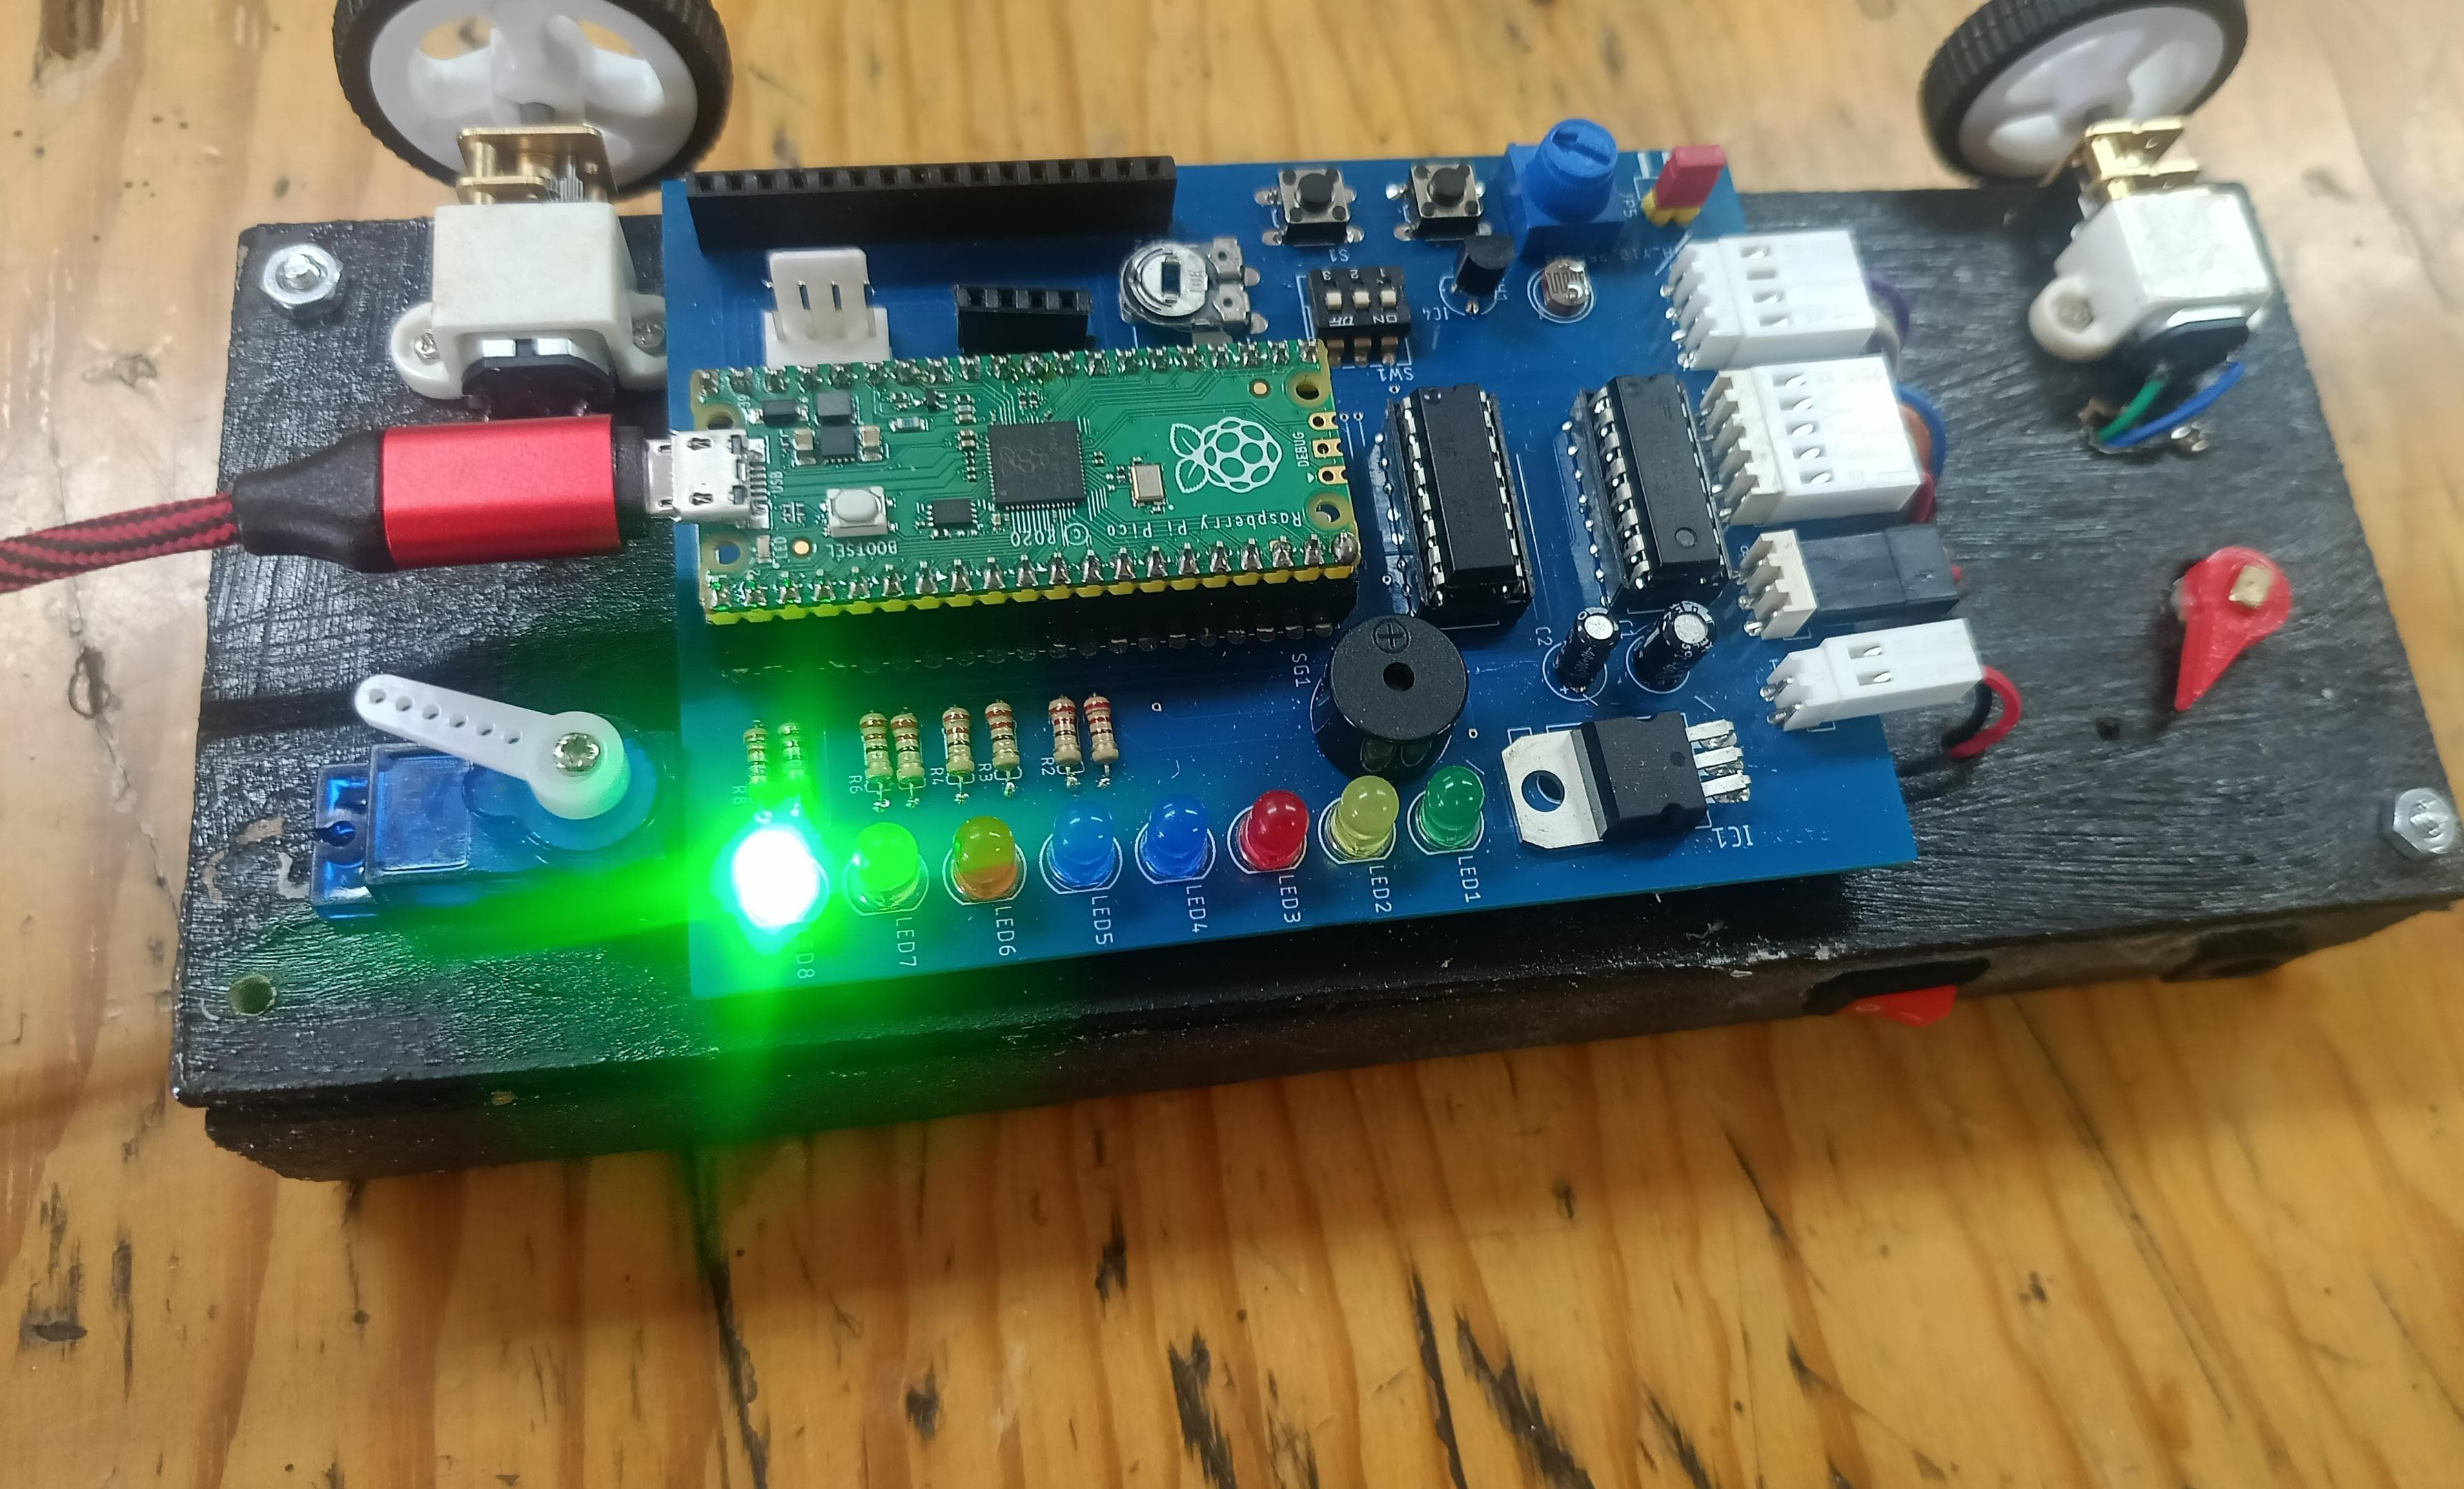
\includegraphics[width=0.7\linewidth]{img/1.jpeg}
    \caption{Tarjeta programada con el Ejercicio 1}
\end{figure}


\subsubsection{Análisis de resultados}
Cuando programamos la tarjeta con el código podemos observar el primer LED color verde prenderse y apagarse en intervalos de medio segundo por lo que el comportamiento es el adecuado al descrito en el código.


%%%%%%%%%%%%%%%%%%%%%%%%%%%%%%%%%%%%%%%%%%%%%%%%%%%%%%%%%%%%%%%%%%%%
\newpage
\subsection{Ejercicio 2}
Realizar las modificaciones necesarias para que los tiempos sean más pequeños y más grandes que el código anterior.

\subsubsection{Pseudo código}

\begin{algorithm}[h]
\SetAlgoLined
\caption{Encendido y apagado del LED con tiempos modificados}

Configurar GPIO0 como salida\;

Mientras verdadero hacer\;
\Indp
Encender LED\;
Esperar 1000 ms\;
Apagar LED\;
Esperar 300 ms\;
\Indm

\end{algorithm}

\subsubsection{Desarrollo}
\begin{lstlisting}
import machine
import utime

# LED de Salida
LED = machine.Pin(0,machine.Pin.OUT)

while True:
    LED.value(1) # LED prendido
    utime.sleep_ms(1000) # 1 segundo de espera
    LED.value(0) # LED apagado
    utime.sleep_ms(300) # 0.3 segundos de espera
\end{lstlisting}

\begin{figure}[h]
    \centering
    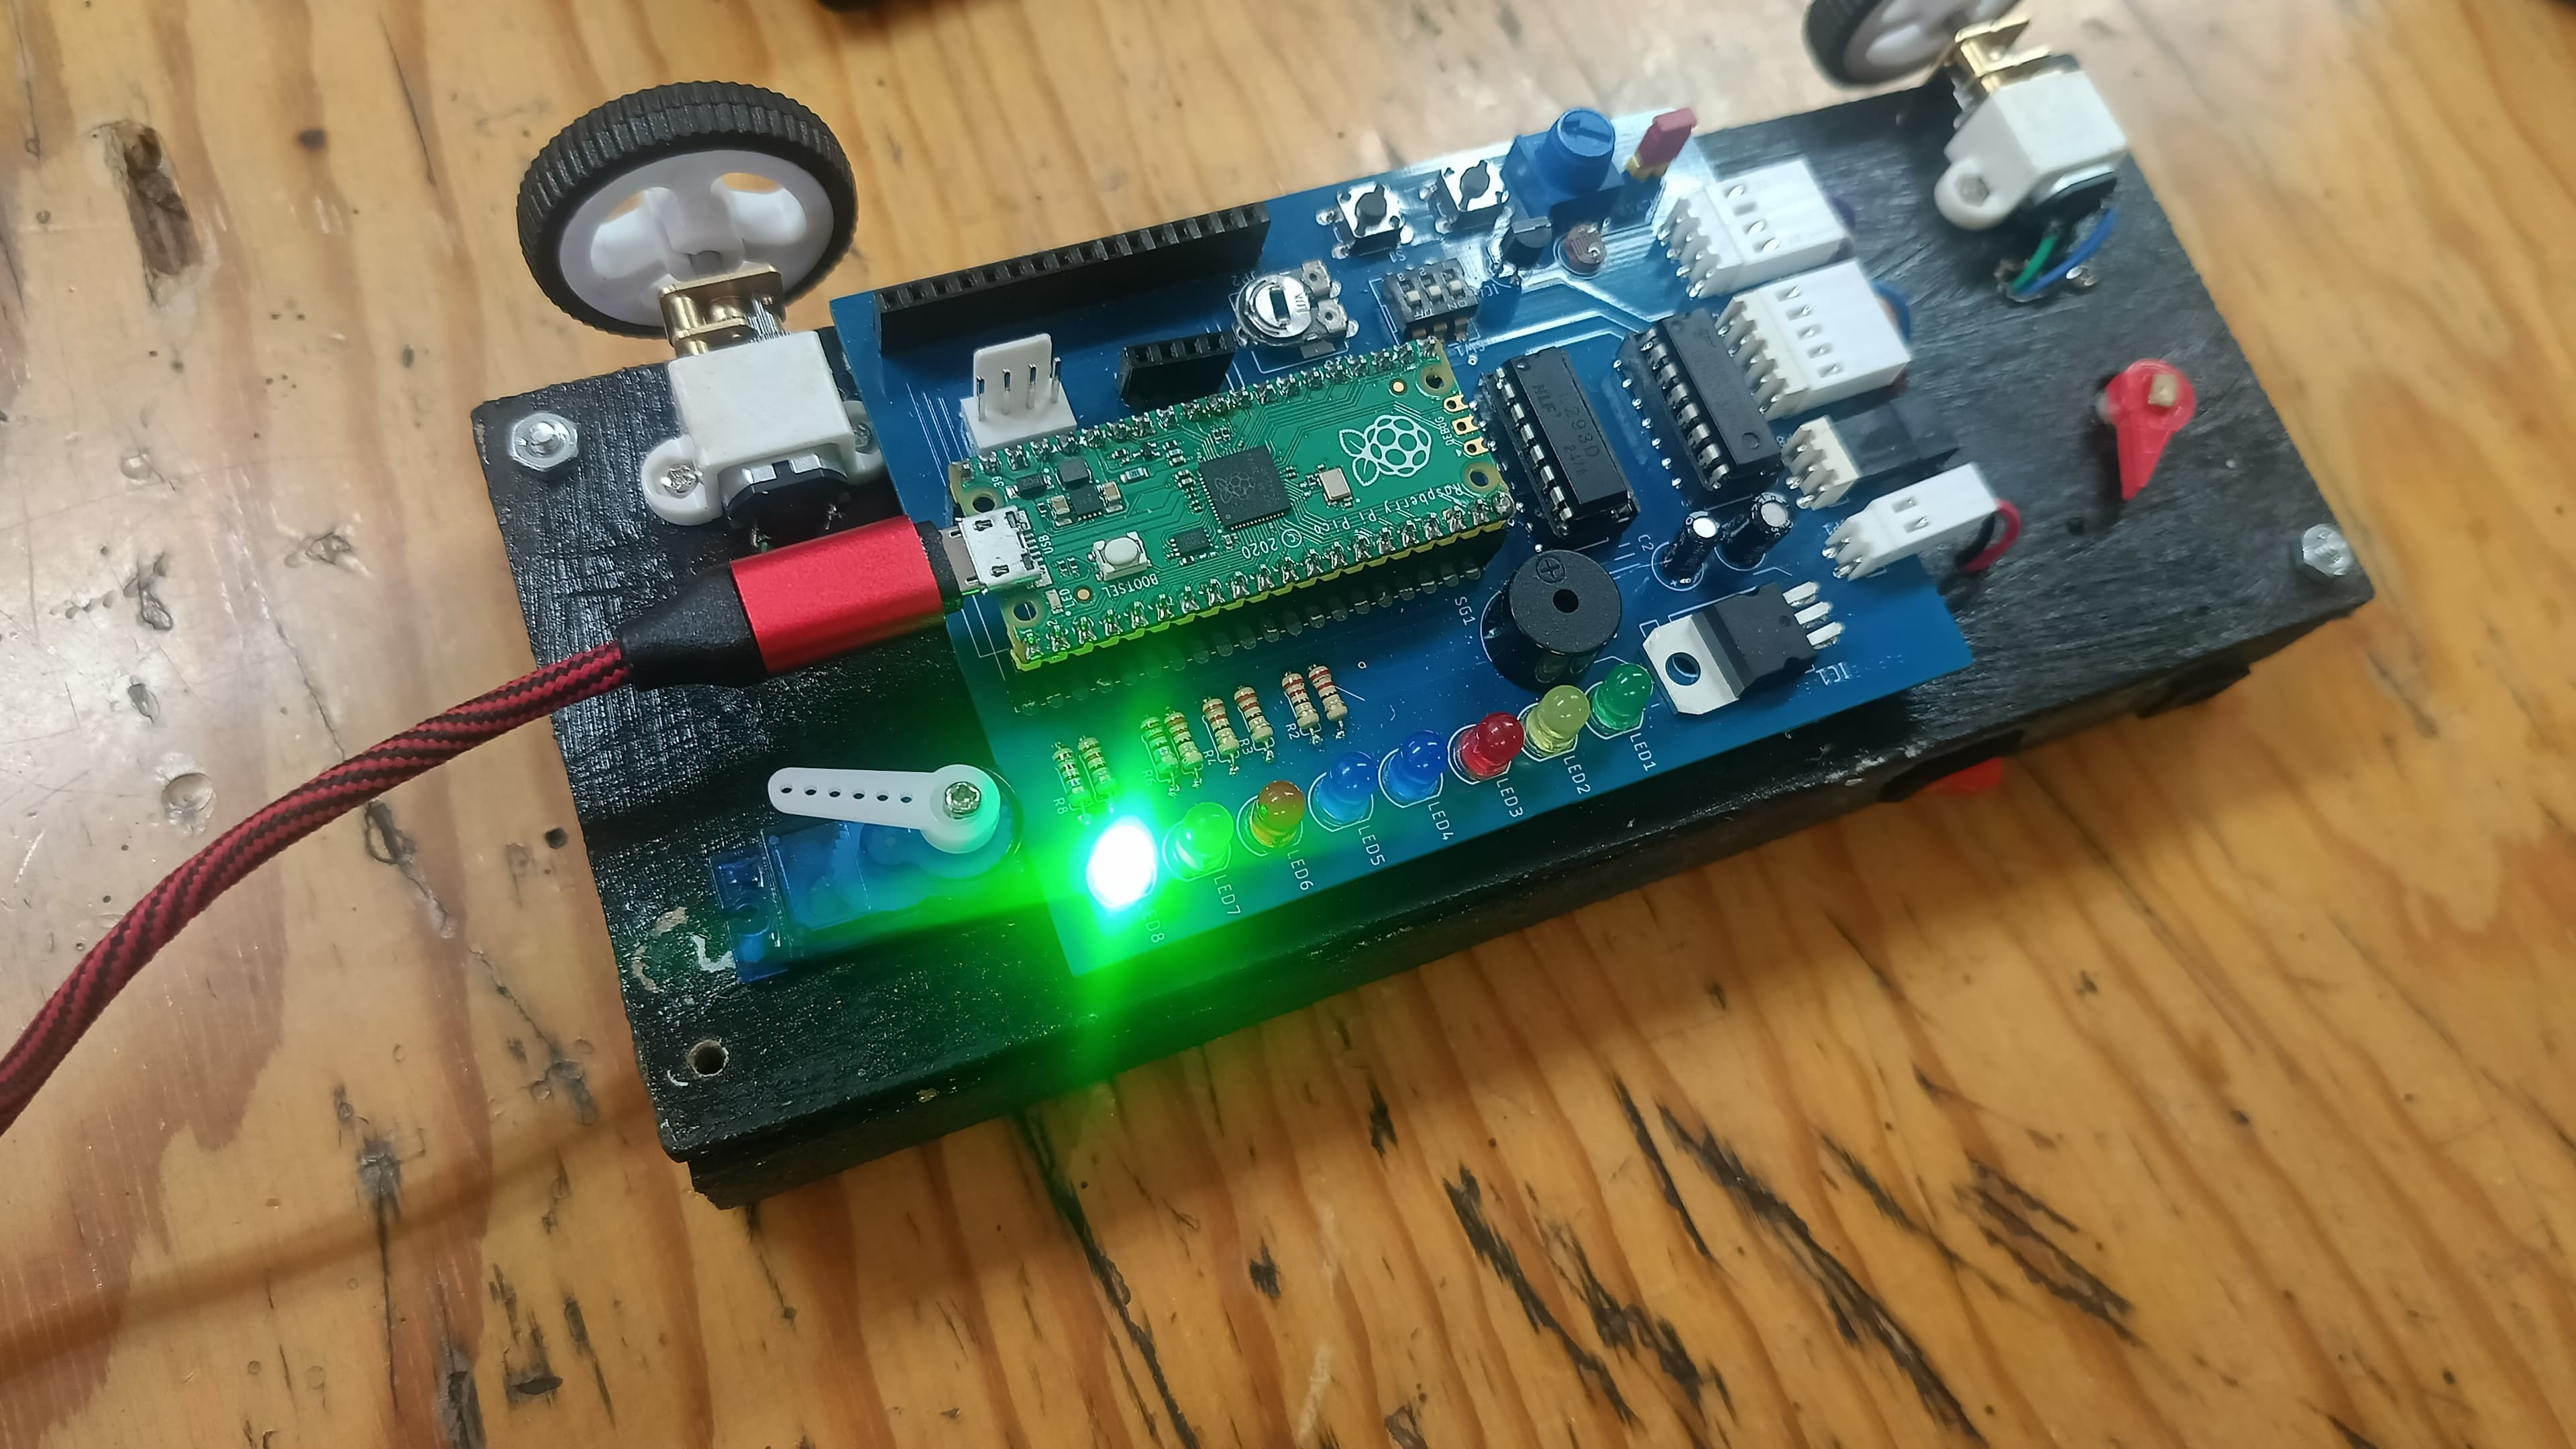
\includegraphics[width=0.7\linewidth]{img/2.jpeg}
    \caption{Tarjeta programada con el Ejercicio 2}
\end{figure}

\subsubsection{Análisis de Resultados}
De manera similar al ejercicio 1, cuando programamos la tarjeta el LED verde prende y apaga pero esta vez permanece prendido durante 1 segundo completo, comportándose de manera adecuado de acuerdo al código escrito.



%%%%%%%%%%%%%%%%%%%%%%%%%%%%%%%%%%%%%%%%%%%%%%%%%%%%%%%%%%%%%%%%%%%%
\newpage
\subsection{Ejercicio 3}
Realizar las modificaciones requeridas para que el efecto se muestre en otro GPIO (podrá usar GPIO1 al GPIO 7); usar retardos a conveniencia.

\subsubsection{Pseudo código}

\begin{algorithm}[h]
\SetAlgoLined
\caption{Control de LED en otro GPIO}

Configurar GPIO2 como salida\;

Mientras verdadero hacer\;
\Indp
Encender LED\;
Esperar 1200 ms\;
Apagar LED\;
Esperar 700 ms\;
\Indm

\end{algorithm}

\subsubsection{Desarrollo}
\begin{lstlisting}
import machine
import utime

# LED de salida
LED = machine.Pin(2,machine.Pin.OUT)

while True:
    LED.value(1) # LED prendido
    utime.sleep_ms(1200) # 1.2 segundos de espera
    LED.value(0) # LED apagado
    utime.sleep_ms(700) # 0.7 segundos de espera
\end{lstlisting}

\begin{figure}[h]
    \centering
    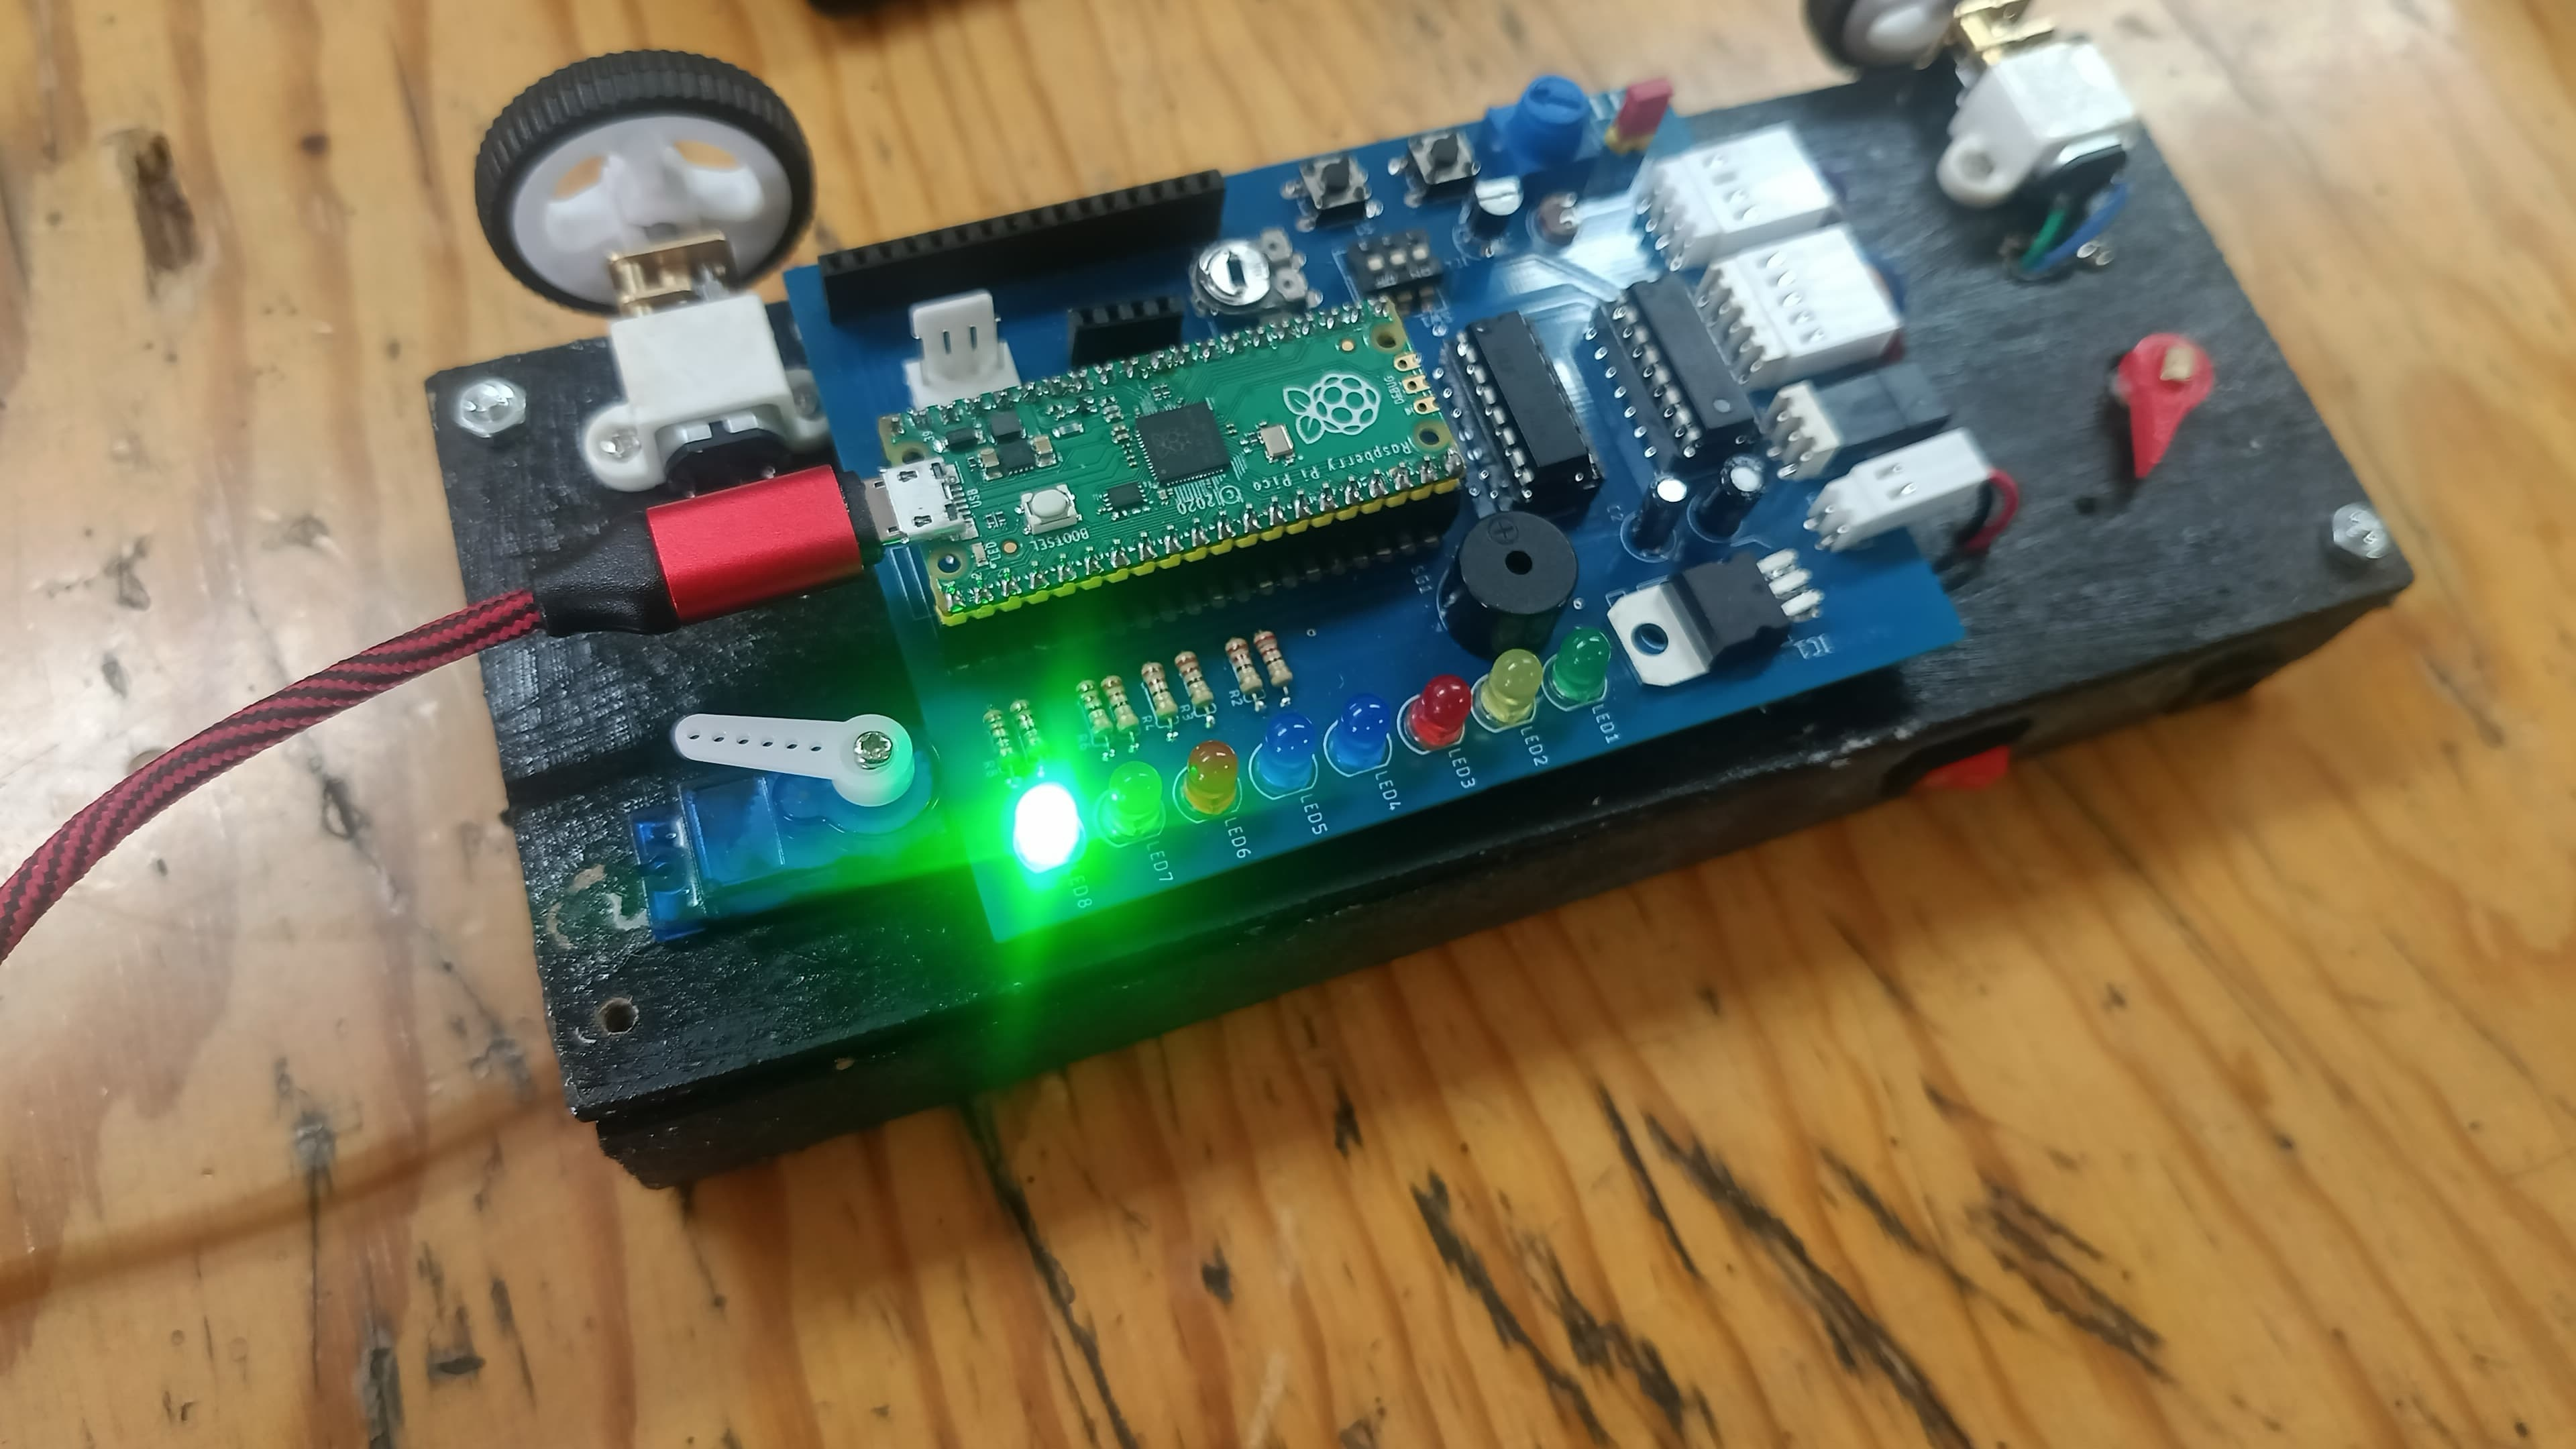
\includegraphics[width=0.7\linewidth]{img/3.jpeg}
    \caption{Tarjeta programada con el Ejercicio 3}
\end{figure}

\subsubsection{Análisis de Resultados}
Una vez más, al programar la tarjeta podemos ver el LED verde prender y apagar con intervalos de 1.2 segundos y 0.7 segundo de acuerdo al código escrito.

%%%%%%%%%%%%%%%%%%%%%%%%%%%%%%%%%%%%%%%%%%%%%%%%%%%%%%%%%%%%%%%%%%%%
\newpage
\subsection{Ejercicio 4}
Realizar un programa que genere las siguientes salidas:

\begin{figure}[h]
    \centering
    
\includegraphics[width=1\linewidth]{pics/Ejercicio4.png}
\end{figure}

\subsubsection{Pseudo código}

\begin{algorithm}[h]
\SetAlgoLined
\caption{Encendido alternado de dos LEDs}

Configurar GPIO2 como salida\;
Configurar GPIO3 como salida\;

Mientras verdadero hacer\;
\Indp
Encender LED en GPIO2\;
Apagar LED en GPIO3\;
Esperar 85 ms\;

Apagar LED en GPIO2\;
Encender LED en GPIO3\;
Esperar 85 ms\;
\Indm

\end{algorithm}
\subsubsection{Desarrollo}
\begin{lstlisting}
import machine
import utime

# LED's de salida
LEDg2 = machine.Pin(2,machine.Pin.OUT)
LEDg3 = machine.Pin(3,machine.Pin.OUT)

while True:
    LEDg2.value(1) # LED rojo prendido
    LEDg3.value(0) # LED azul apagado
    utime.sleep_ms(85) # 0.085 segundos de espera
    LEDg2.value(0) # LED rojo apagado
    LEDg3.value(1) # LED azul prendido
    utime.sleep_ms(85) # 0.085 segundos de espera
\end{lstlisting}

\newpage
\begin{figure}[h]
    \centering
    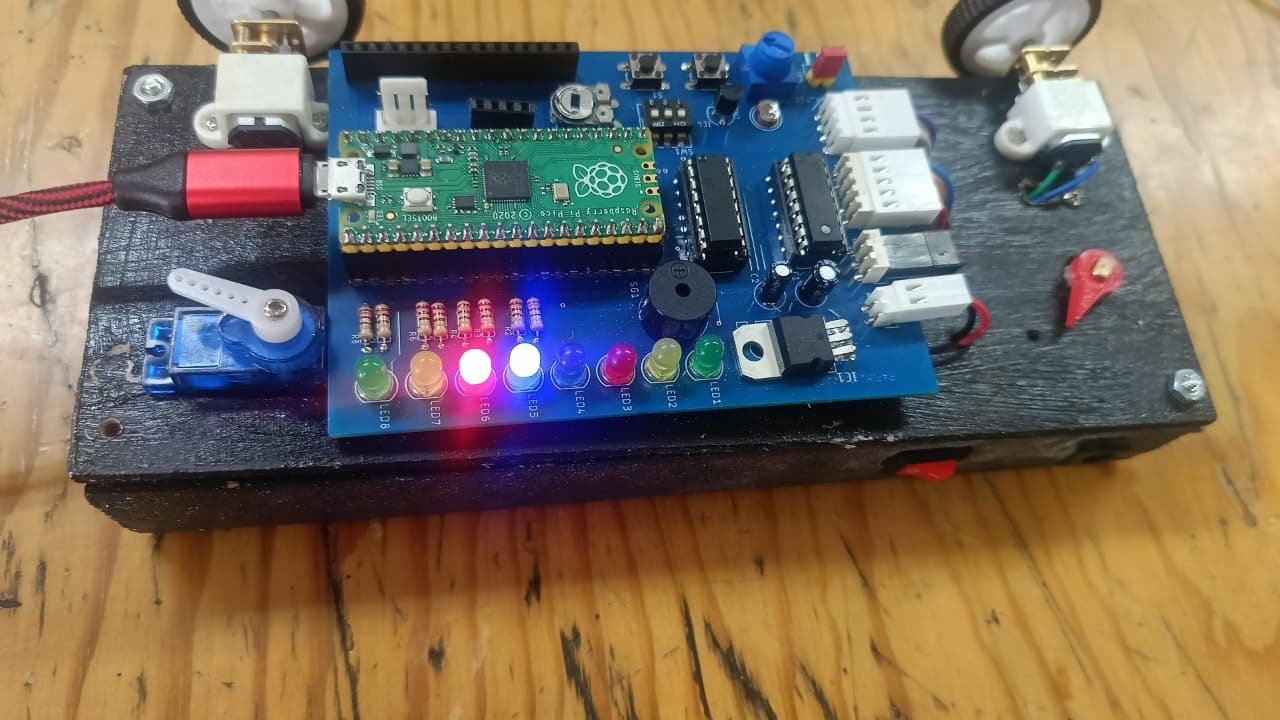
\includegraphics[width=0.7\linewidth]{img/4.jpeg}
    \caption{Tarjeta programada con el Ejercicio 4}
\end{figure}

\subsubsection{Análisis de Resultados}
Al programar la tarjeta observamos como el LED rojo y azul cambian estados de prendido a apagado intercaladamente siguiendo el comportamiento descrito en el código de manera correcta.

%%%%%%%%%%%%%%%%%%%%%%%%%%%%%%%%%%%%%%%%%%%%%%%%%%%%%%%%%%%%%%%%%%%%
\newpage
\subsection{Ejercicio 5}
Realizar un programa que prenda y apague las GPIO0 al GPIO7; el circuito corresponde en su totalidad al mostrado en la figura 3.3, usar los retardos a elección
\begin{figure}[h]
    \centering
    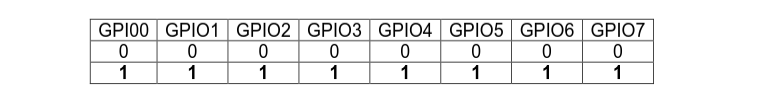
\includegraphics[width=1\linewidth]{pics/Ejercicio5.png}
\end{figure}

\subsubsection{Pseudo código}

\begin{algorithm}[h]
\SetAlgoLined
\caption{Encendido y apagado simultáneo de GPIO0 a GPIO7}

Definir lista de GPIO del 0 al 7\;

Mientras verdadero hacer\;
\Indp

Para cada LED en la lista hacer\;
\Indp
Encender LED\;
\Indm

Esperar 800 ms\;

Para cada LED en la lista hacer\;
\Indp
Apagar LED\;
\Indm

Esperar 800 ms\;

\Indm
\end{algorithm}

\subsubsection{Desarrollo}
\begin{lstlisting}
import machine
import utime

# LED's de salida
numero_pin = [0, 1, 2, 3, 4, 5, 6, 7]
leds = [machine.Pin(p, machine.Pin.OUT) for p in numero_pin]

while True:
    # Prender todos los LED's
    for led in leds:
        led.value(1)
    utime.sleep_ms(800) # 0.8 segundos de espera

    # Apagadar todos los LED's
    for led in leds:
        led.value(0)
    utime.sleep_ms(800) # 0.8 segundos de espera
\end{lstlisting}

\newpage
\begin{figure}[h]
    \centering
    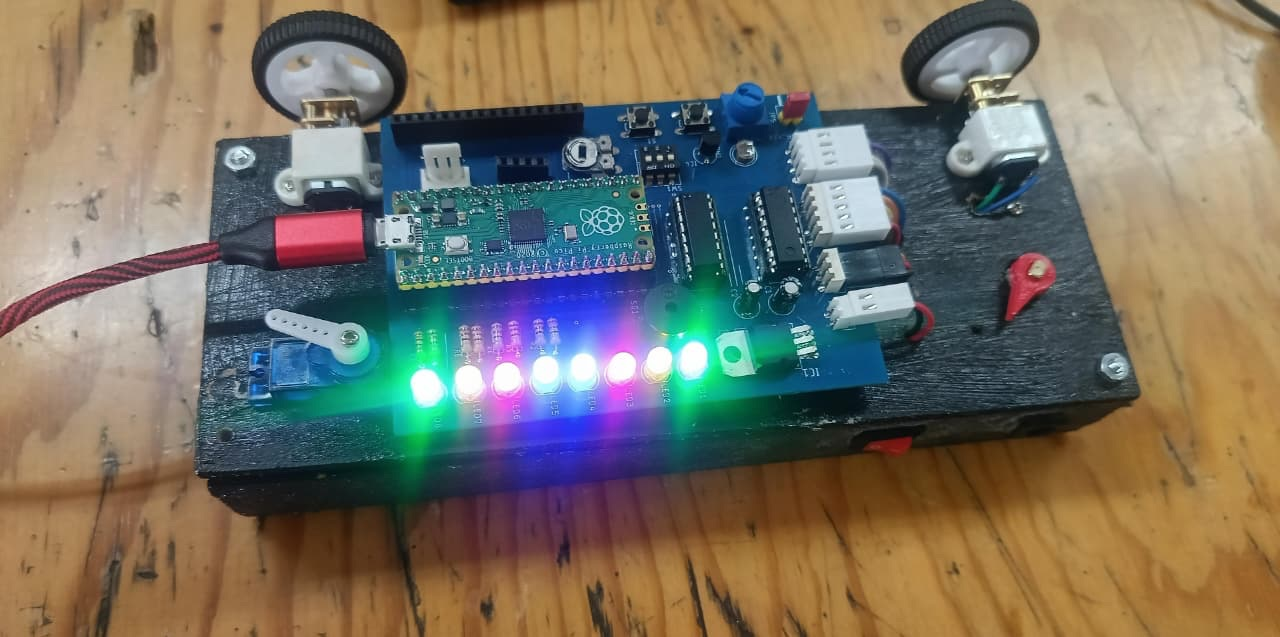
\includegraphics[width=0.7\linewidth]{img/5.jpeg}
    \caption{Tarjeta programada con el Ejercicio 5}
\end{figure}

\subsubsection{Análisis de Resultados}
Al ejecutar el programa en la tarjeta podemos observar que los 8 LED's prenden simultáneamente y también se apagan simultáneamente de manera acorde al código.

%%%%%%%%%%%%%%%%%%%%%%%%%%%%%%%%%%%%%%%%%%%%%%%%%%%%%%%%%%%%%%%%%%%%
\newpage
\subsection{Ejercicio 6}
Repetir la acción anterior 10 veces; mantener apagado 2 segundos y repetir acción.
\begin{figure}[h]
    \centering
    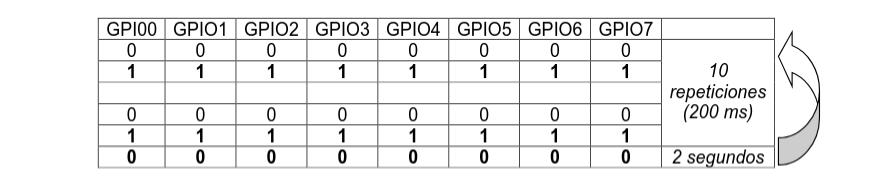
\includegraphics[width=0.9\linewidth]{pics/Ejercicio6.png}
\end{figure}

\subsubsection{Pseudo código}

\begin{algorithm}[h]
\SetAlgoLined
\caption{Encendido y apagado de LEDs repetido 10 veces}

Definir lista de GPIO del 0 al 7\;

Mientras verdadero hacer\;
\Indp

Repetir 10 veces\;
\Indp

Para cada LED en la lista hacer\;
\Indp
Encender LED\;
\Indm

Esperar 200 ms\;

Para cada LED en la lista hacer\;
\Indp
Apagar LED\;
\Indm

Esperar 200 ms\;

\Indm

Esperar 2000 ms\;

\Indm
\end{algorithm}

\subsubsection{Desarrollo}
\begin{lstlisting}
import machine
import utime

# LED's de salida
numero_pin = [0, 1, 2, 3, 4, 5, 6, 7]
leds = [machine.Pin(p, machine.Pin.OUT) for p in numero_pin]

# Tiempos de retardo
retardo_rep = 200
retardo_espera = 2000

while True:
    # 10 repeticiones
    for i in range(10):
        # Prender todos los LED's
        for led in leds:
            led.value(1)
        utime.sleep_ms(retardo_rep) # 0.2 segundos de espera

        # Apagar todos los LED's
        for led in leds:
            led.value(0)
        utime.sleep_ms(retardo_rep) # 0.2 segundos de espera
    
    # Fin de las 10 repeticiones
    utime.sleep_ms(retardo_espera) # 2 segundos de espera
\end{lstlisting}

\begin{figure}[h]
    \centering
    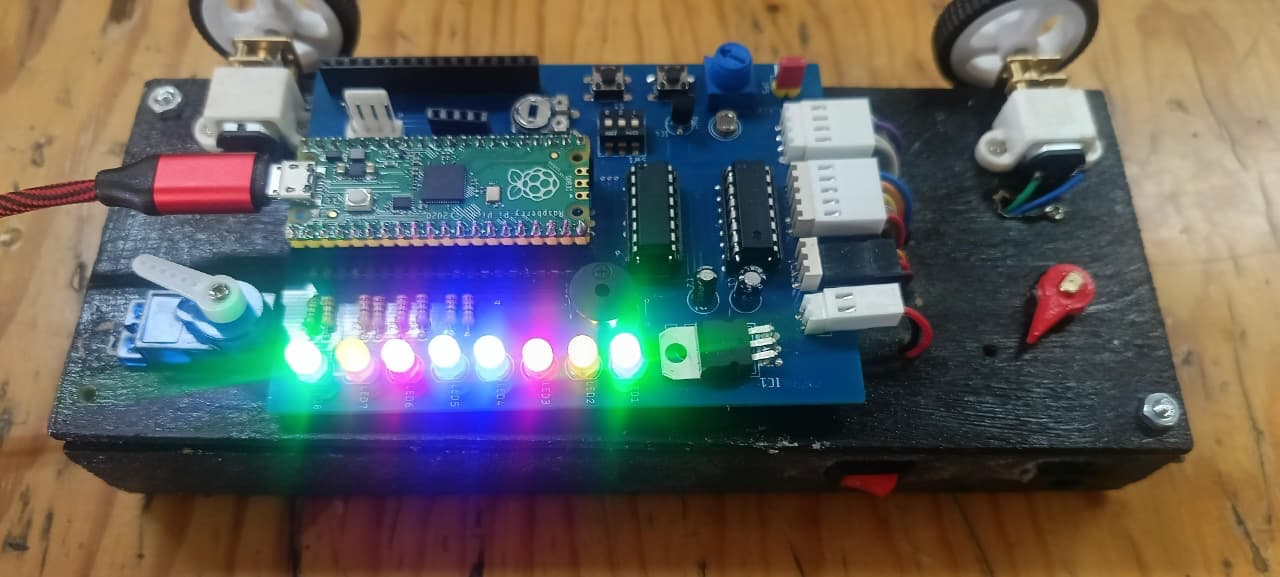
\includegraphics[width=0.7\linewidth]{img/6.jpeg}
    \caption{Tarjeta programada con el Ejercicio 6}
\end{figure}

\subsubsection{Análisis de Resultados}
Al programar la tarjeta podemos observar 8 LED's prenderse y apagarse simultáneamente un total de 10 veces con intervalos de 0.2 segundos y al finalizar las 10 repeticiones hay un tiempo de espera de 2 segundos antes de comenzar nuevamente con las 10 repeticiones, de forma que el comportamiento descrito por el código se ejecuta correctamente.

%%%%%%%%%%%%%%%%%%%%%%%%%%%%%%%%%%%%%%%%%%%%%%%%%%%%%%%%%%%%%%%%%%%%
\newpage
\subsection{Ejercicio 7}
Usando los GPIO0 al GPIO7; realizar un programa que genere la siguiente secuencia; usar retardos de 100ms.
\begin{figure}[h]
    \centering
    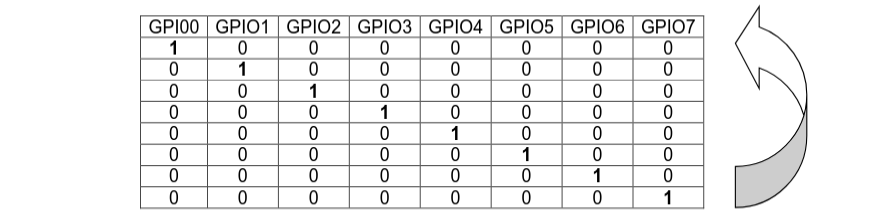
\includegraphics[width=1\linewidth]{pics/Ejercicio7.png}
\end{figure}

\subsubsection{Pseudo código}

\begin{algorithm}[h]
\SetAlgoLined
\caption{Encendido secuencial de LEDs}

Definir lista de GPIO del 0 al 7\;

Mientras verdadero hacer\;
\Indp

Para cada LED en la lista hacer\;
\Indp
Encender LED\;
Esperar 100 ms\;
Apagar LED\;
\Indm

\Indm
\end{algorithm}

\subsubsection{Desarrollo}
\begin{lstlisting}
import machine
import utime

# LED's de salida
numero_pin = [0, 1, 2, 3, 4, 5, 6, 7]
leds = [machine.Pin(p, machine.Pin.OUT) for p in numero_pin]

retardo = 100 # Tiempo de retard

while True:
    for led in leds:
        led.value(1) # LED prendido
        utime.sleep_ms(retardo) # 0.1 segundos de espera
        led.value(0) # LED apagado
\end{lstlisting}

\newpage
\begin{figure}[h]
    \centering
    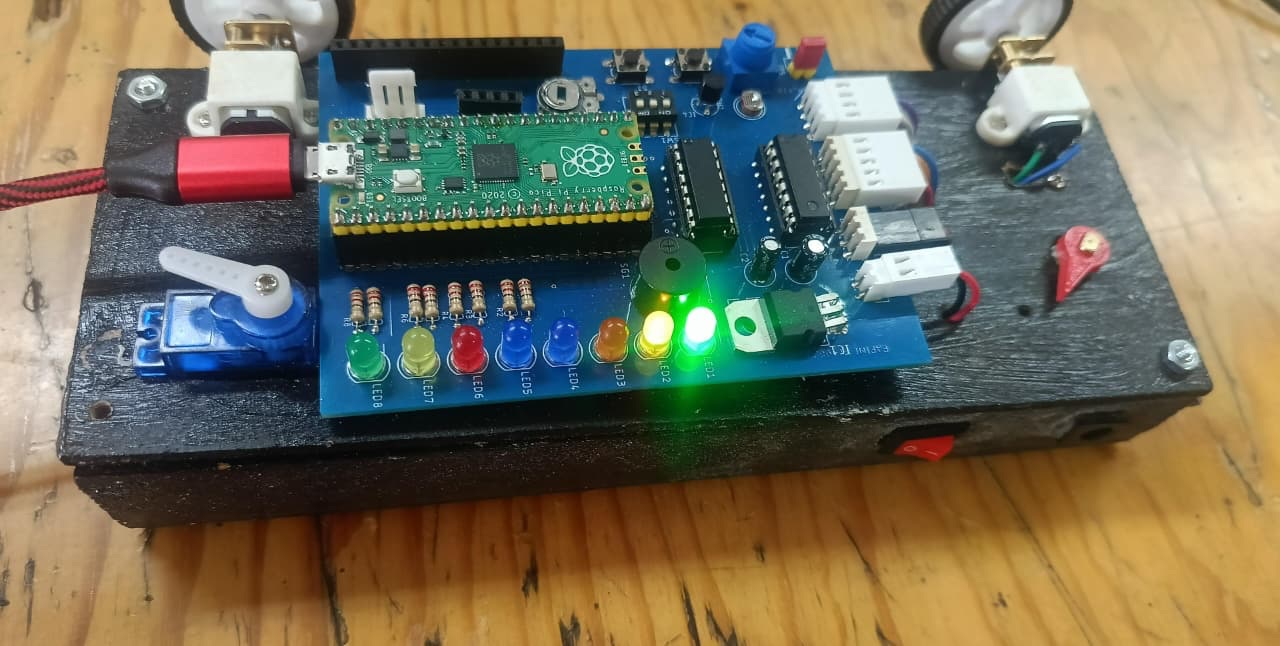
\includegraphics[width=0.7\linewidth]{img/7.jpeg}
    \caption{Tarjeta programada con el Ejercicio 7}
\end{figure}

\subsubsection{Análisis de Resultados}
Al programar la tarjeta con este código se observa que los 8 LED's se encienden uno tras otro de forma secuencial comenzando desde el GPIO0 hasta el GPIO7. Cada LED permanece encendido durante 100 ms antes de apagarse y continuar con el siguiente LED en la secuencia. Este comportamiento genera un efecto visual de desplazamiento de luz a lo largo de los LEDs, confirmando que el ciclo \texttt{for} recorre correctamente la lista de pines y que los retardos se ejecutan de acuerdo con el tiempo establecido en el programa.


%%%%%%%%%%%%%%%%%%%%%%%%%%%%%%%%%%%%%%%%%%%%%%%%%%%%%%%%%%%%%%%%%%%%
\newpage
\subsection{Ejercicio 8}
Usando los GPIO0 al GPIO7; realizar un programa que genere la siguiente secuencia; usar retardos de 100ms.
\begin{figure}[h]
    \centering
    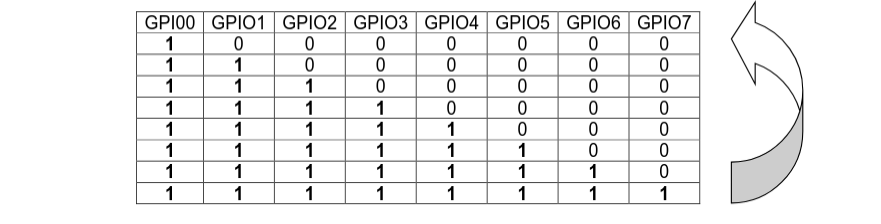
\includegraphics[width=1\linewidth]{pics/Ejercicio8.png}
\end{figure}

\subsubsection{Pseudo código}

\begin{algorithm}[h]
\SetAlgoLined
\caption{Encendido progresivo de LEDs}

Definir lista de GPIO del 0 al 7\;

Mientras verdadero hacer\;
\Indp

Para i desde 0 hasta 7 hacer\;
\Indp

Para j desde 0 hasta i hacer\;
\Indp
Encender LED j\;
\Indm

Esperar 100 ms\;

\Indm

Apagar todos los LEDs\;

\Indm
\end{algorithm}

\subsubsection{Desarrollo}
\begin{lstlisting}
import machine
import utime

numero_pin = [0, 1, 2, 3, 4, 5, 6, 7]
leds = [machine.Pin(p, machine.Pin.OUT) for p in numero_pin]

retardo = 100

while True:
    for i in range(len(leds)):
        for j in range(i+1):
            leds[j].value(1)
        utime.sleep_ms(retardo)

    for led in leds:
        led.value(0)
\end{lstlisting}

\newpage
\begin{figure}[h]
    \centering
    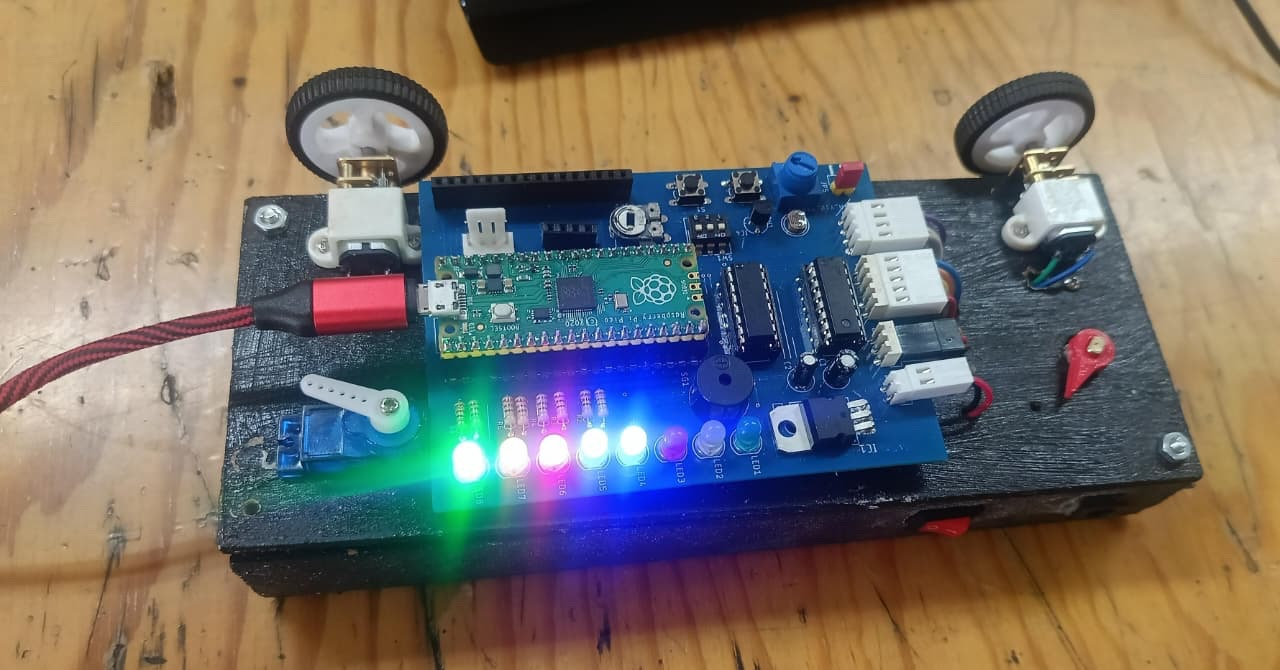
\includegraphics[width=0.7\linewidth]{img/8.jpeg}
    \caption{Tarjeta programada con el Ejercicio 8}
\end{figure}

\subsubsection{Análisis de Resultados}
Al ejecutar el programa en la tarjeta se observa que los LED's se encienden de forma progresiva. Primero se enciende el primer LED, posteriormente el segundo manteniendo encendido el anterior, y así sucesivamente hasta que los ocho LED's permanecen encendidos al mismo tiempo. Después de completar la secuencia, todos los LED's se apagan y el proceso se repite nuevamente. Este comportamiento confirma que el uso de los ciclos anidados permite controlar el encendido acumulativo de los LEDs conforme a lo especificado en el código.


%%%%%%%%%%%%%%%%%%%%%%%%%%%%%%%%%%%%%%%%%%%%%%%%%%%%%%%%%%%%%%%%%%%%
\newpage
\subsection{Ejercicio 9}
Usando los GPIO0 al GPIO7; realizar un programa que genere un contador de 8 bits de forma ascendente; usar retardos de 50ms.
\begin{figure}[h]
    \centering
    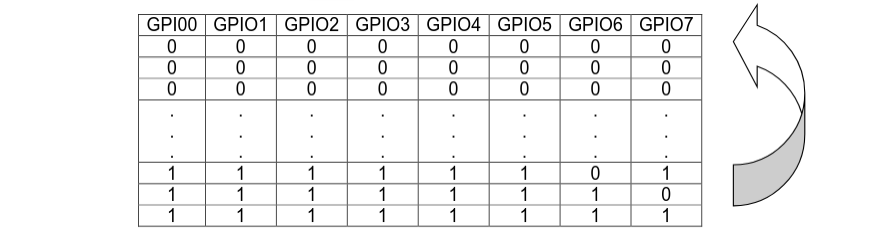
\includegraphics[width=1\linewidth]{pics/Ejercicio9.png}
\end{figure}

\subsubsection{Pseudo código}

\begin{algorithm}[h]
\SetAlgoLined
\caption{Contador binario de 8 bits}

Definir lista de GPIO del 0 al 7\;

Mientras verdadero hacer\;
\Indp

Para numero desde 0 hasta 255 hacer\;
\Indp

Para bit desde 0 hasta 7 hacer\;
\Indp
Obtener valor del bit correspondiente del número\;
Asignar valor al LED correspondiente\;
\Indm

Esperar 50 ms\;

\Indm

\Indm
\end{algorithm}

\subsubsection{Desarrollo}
\begin{lstlisting}
import machine
import utime

numero_pin = [0, 1, 2, 3, 4, 5, 6, 7]
leds = [machine.Pin(p, machine.Pin.OUT) for p in numero_pin]

retardo = 50

while True:
    for numero in range(256):
        for bit in range (8):
            estado_bit = (numero >> bit) & 1
            leds[7-bit].value(estado_bit)
        utime.sleep_ms(retardo)
\end{lstlisting}

\newpage
\begin{figure}[h]
    \centering
    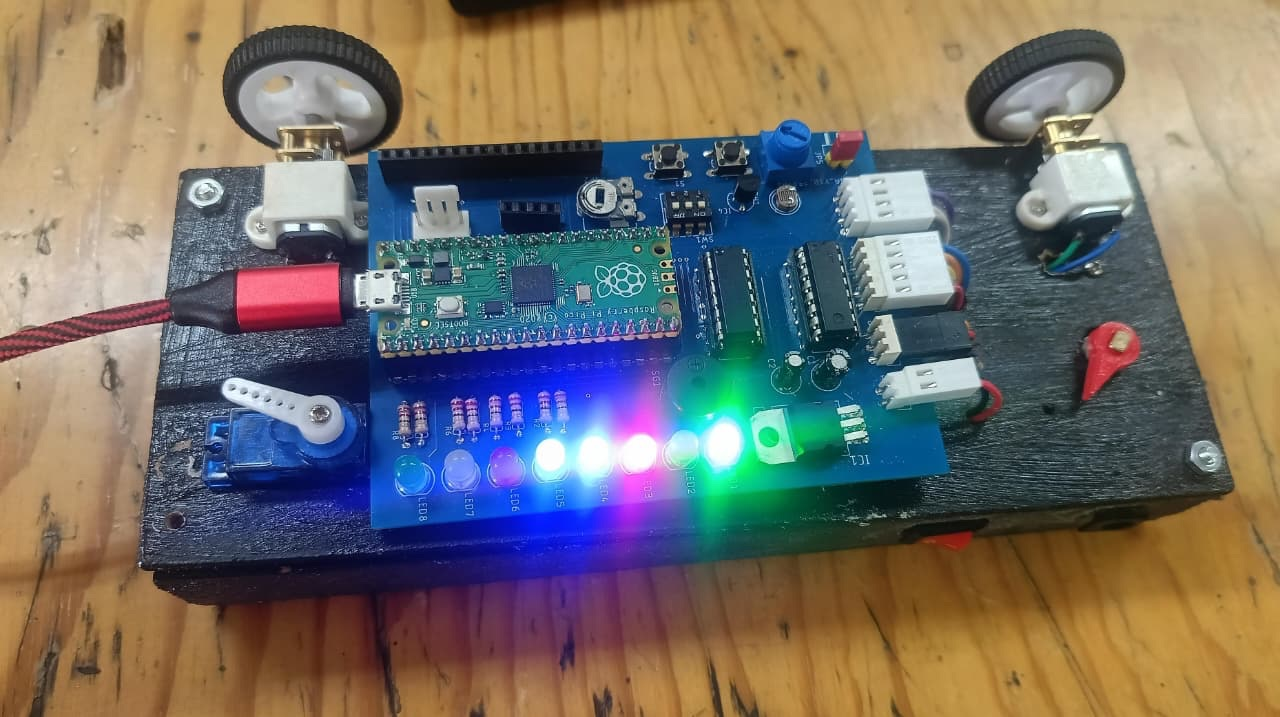
\includegraphics[width=0.7\linewidth]{img/9.jpeg}
    \caption{Tarjeta programada con el Ejercicio 9}
\end{figure}

\subsubsection{Análisis de Resultados}
Al cargar el programa en la tarjeta se observa que los LED's representan visualmente un contador binario de 8 bits. Los LEDs cambian de estado cada 50 ms mostrando las diferentes combinaciones binarias desde 00000000 hasta 11111111, lo cual corresponde a los valores decimales del 0 al 255. Este comportamiento permite verificar que la operación de desplazamiento de bits y la asignación de cada bit a un LED funcionan correctamente, generando una representación visual del conteo binario ascendente.


%%%%%%%%%%%%%%%%%%%%%%%%%%%%%%%%%%%%%%%%%%%%%%%%%%%%%%%%%%%%%%%%%%%%
\newpage
\subsection{Ejercicio 10}
Usando las salidas correspondientes a los colores de los leds; realizar un programa que controle el funcionamiento de dos semáforos, de acuerdo a la siguiente tabla.
\begin{figure}[h]
    \centering
    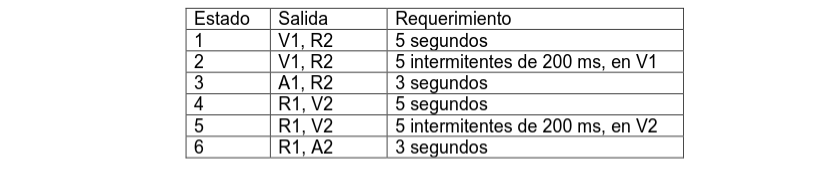
\includegraphics[width=1\linewidth]{pics/Ejercicio10.png}
\end{figure}

\subsubsection{Pseudo código}

\begin{algorithm}[h]
\SetAlgoLined
\caption{Control de dos semáforos}

Configurar pines de semáforo 1 (V1, A1, R1)\;
Configurar pines de semáforo 2 (V2, A2, R2)\;

Mientras verdadero hacer\;
\Indp

Encender V1 y R2\;
Esperar 5 s\;

Repetir 5 veces\;
\Indp
Apagar V1\;
Esperar 200 ms\;
Encender V1\;
Esperar 200 ms\;
\Indm

Apagar V1\;
Encender A1 y R2\;
Esperar 3 s\;

Encender R1 y V2\;
Esperar 5 s\;

Repetir 5 veces\;
\Indp
Apagar V2\;
Esperar 200 ms\;
Encender V2\;
Esperar 200 ms\;
\Indm

Apagar V2\;
Encender A2 y R1\;
Esperar 3 s\;

\Indm
\end{algorithm}

\newpage
\subsubsection{Desarrollo}
\begin{lstlisting}
import machine
import utime

V1 = machine.Pin(0, machine.Pin.OUT)
A1 = machine.Pin(1, machine.Pin.OUT)
R1 = machine.Pin(2, machine.Pin.OUT)

V2 = machine.Pin(7, machine.Pin.OUT)
A2 = machine.Pin(6, machine.Pin.OUT)
R2 = machine.Pin(5, machine.Pin.OUT)

while True:
    R1.value(0)
    A2.value(0)
    #E1: V1 y R2 prendidos 5 seg
    V1.value(1)
    R2.value(1)
    utime.sleep_ms(5000)

    #E2: V1 5 intermitentes 200ms, R2 prendido
    for i in range(5):
        V1.value(0)
        utime.sleep_ms(200)
        V1.value(1) 
        utime.sleep_ms(200)    

    #E3: A1 y R2 prendido 3 seg
    V1.value(0)
    A1.value(1)
    utime.sleep_ms(3000)

    #E4: R1 y V2 prendidos 5 seg
    A1.value(0)
    R1.value(1)
    R2.value(0)
    V2.value(1)
    utime.sleep_ms(5000)

    #E5: V2 5 intermitentes 200ms, R1 prendido
    for i in range(5):
        V2.value(0)
        utime.sleep_ms(200)
        V2.value(1) 
        utime.sleep_ms(200) 
    
    #E6: R1 y A2 prendidos 3 seg
    V2.value(0)
    A2.value(1)
    utime.sleep_ms(3000)
\end{lstlisting}

\newpage
\begin{figure}[h]
    \centering
    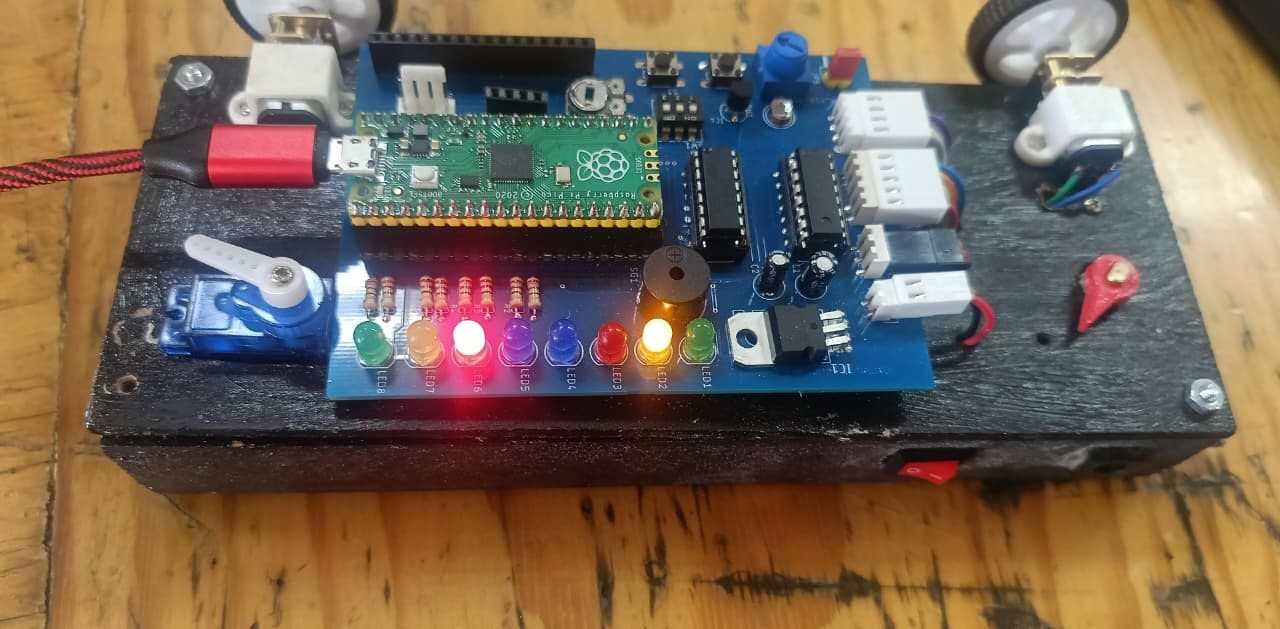
\includegraphics[width=0.7\linewidth]{img/10.jpeg}
    \caption{Tarjeta programada con el Ejercicio 10}
\end{figure}

\subsubsection{Análisis de Resultados}
Al ejecutar el programa se observa el funcionamiento de dos semáforos que operan de manera alternada simulando un cruce vehicular. Inicialmente el semáforo 1 permanece en verde mientras el semáforo 2 se encuentra en rojo durante 5 segundos. Posteriormente el LED verde del semáforo 1 parpadea indicando el cambio próximo a amarillo, el cual permanece encendido durante 3 segundos antes de pasar a rojo. En ese momento el semáforo 2 cambia a verde y se repite el mismo proceso de parpadeo y cambio a amarillo. Este comportamiento demuestra que la lógica de control implementada en el código permite coordinar correctamente las fases de ambos semáforos.
